\documentclass[11pt, a4paper]{article}
\usepackage{geometry}
\geometry{
 a4paper,
 total={170mm,257mm},
 left=2cm,
 top=2cm,
 right= 2cm,
 bottom = 2cm
 }
\usepackage{glossaries}
\usepackage{graphicx}
\usepackage{amsmath}
\usepackage{siunitx}
\usepackage{subcaption}
\usepackage{url}
\usepackage{flafter}
\usepackage{float}
\usepackage{tabularx}
\usepackage[section]{placeins}
\usepackage{subcaption}
\usepackage[utf8]{inputenc}
\usepackage{setspace} 
\doublespacing{}
\usepackage[
backend=biber,
style=numeric,
sorting=ynt
]{biblatex}
\addbibresource{mybibliography.bib}
\makenoidxglossaries{}

\newglossaryentry{Static air}
{
    name=Static air,
    description={Air that is not moving in any direction. The wind speed is 0km/h}
}
\newglossaryentry{Coanda effect}
{
    name=coanda effect,
    description={The tendency of a fluid to stay attached to a convex surface}
}
\newglossaryentry{Grip}
{
    name=grip,
    description={Friction available between the tyres of a car and the track surface, \\ defined by the formula \(F=\mu*(m*(g+R))\) where \(R\Rightarrow Downforce[units: N]\)}
}
\newglossaryentry{AWS}
{
    name=Absolute Wind Speed,
    description={The speed of wind (in km/h) on the track. The speed of wind measurred by an anemometer. For the purpose of this research, AWS is assigned the symbol \(w_A\). A positive value signifies headwind, negative is tailwind, while \(0km/h\) is no wind}
}
\newglossaryentry{RWS}
{
    name=Relative Wind Speed,
    description={The speed of wind (in km/h) on the track, AWS, plus the velocity of the car. For the purpose of this research, RWS is assigned the symbol \(w_R\), defined as \(w_A=v+w_A\)}
}
\newglossaryentry{AoA}
{
    name=Angle of Attack,
    description={
        AoA is the angle of the wing with respect ot the streamlined wind flow. The higher the AoA, more downforce and hence more drag is produced. Until a certain point where downforce production
        decreases while drag production still increases. This effect is alled stalling. 
        \begin{center}
            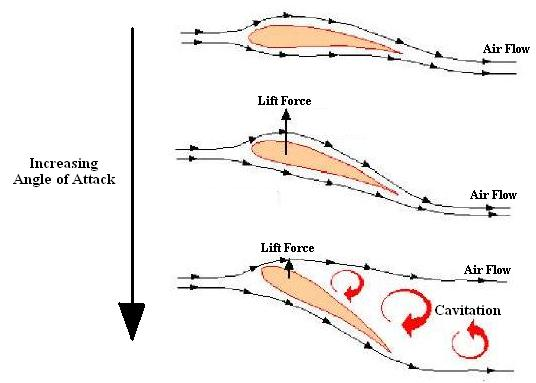
\includegraphics[width=\textwidth]{images/angleOfAttack.jpg}\newline
        \end{center}    
        Image source: http://www.somersf1.co.uk/p/angle-of-attack-aoa-f1-technical-terms.html
    }
}
\newglossaryentry{Headwind}
{
    name=headwind,
    description={
        wind that is going the opposite direction of movement. For headwind, \gls{AWS} and \gls{RWS} are positive.
    }
}
\newglossaryentry{Tailwind}
{
    name=tailwind,
    description={
        wind that is going the same direction of movement. For tailwind, \gls{AWS} and \gls{RWS} are negative.
    }
}
\title{\textbf{Subject: Physics} \\[1ex] \Large \underline{Analyzing the relationship between Speed and Downforce, and Drag in a race car} \\ \large RQ: How does a velocity of a car affect the aerodynamic drag and downforce acting on the rear wing with an Angle of Attack at $21.4^{\circ}$?
}
\date{Word Count:3900\\Personal Code: lch068}
%TODO: word count\date{word}
\begin{document}
\maketitle

\newpage
\tableofcontents
\clearpage
\section{Introduction}
\subsection{Source of motivation}
I have been fascinated by cars ever since I was a child. I enjoyed learning about the mechanical engineering that goes behind car manufacturing, let alone making a race car. But what
specifically caught my interest was the shape of these vehicles. It is quite known that cars that are sleeker move faster than cars with orthogonal geometries. But looking at the car structures in a Formula 1 race,
I noticed that although their general shape is very similar, looking closely at the body, front wing, rear wing very slight changes can be seen. Every slight change in curvature of the body could result in significant changes in performance.
\\\\
Aerodynamics can be very helpful, not only in terms of faster race cars and better racing which improve the entertainment sector, but also improving efficiency of cars, boats and planes. Car manufacturers, implement the knowledge gained from
their motorsports division and apply it to their production vehicles. Making cars not only go faster but improving the economy of the car. These changes have been a major factor in the evolution of road cars over the years.
Additionally, understanding the relationship between drag and car velocity could help to design a clever engine cooling system.
Production cars are usually cooled by the air intake from the front grill, but the block shapped parts of the engine can significantly increase drag.
Understanding the latter relationship helps decide to what extent can one increase the drag coefficient of the car without resulting in loss of performance.
\\\\
The aim of this experiment is to understand how the fundamental aerodynamic forces acting on a race car can affect its performance. This research aims to answer the following research question:
\subsection{Research Question}
How does a velocity of a car affect the aerodynamic drag and downforce acting on the rear wing with an Angle of Attack at $21.4^{\circ}$? 
%\subsection{Hypothesis}
%As the aerodynamic force is expected to increase with car speed
%the rate of change of downforce must be higher than of drag. This is because the drivers are aware that going faster will increase their downforce and drag, 
%and yet Formula 1 drivers choose to go at higher speed from the beginning, which shows that they
%prioritize downforce over drag.
%\subsection{Application of Aerodynamic Studies}
%Aerodynamics can be very helpful, not only in terms of faster race cars and better racing which improve the entertainment sector, but also improving efficiency of cars, boats and planes. 
%Car manufacturers, especially those that compete in Formula 1, learn a lot about aerodynamics from their Formula 1 teams and implement them in their road cars. Making cars not only go faster
%but improving the economy of the car. 
%The conclusions of the research question may help answer whether a manufacturer should prioritize downforce over drag to achieve maximmum overall laptime.

\section{Background Knowledge}
When an object is moving through space 4 specific forces act on it. These forces are Thrust, Gravitational force
Drag force and Lift/Downforce. \textit{figure~\ref{fig:freeBodyDiagram}} represents a freebody diagram of these forces acting on a teardrop-shaped object moving through air with a constant velocity.
\begin{figure}[H]
    \caption{Free Body Diagram of teardrop object moving with }
    \centering 
    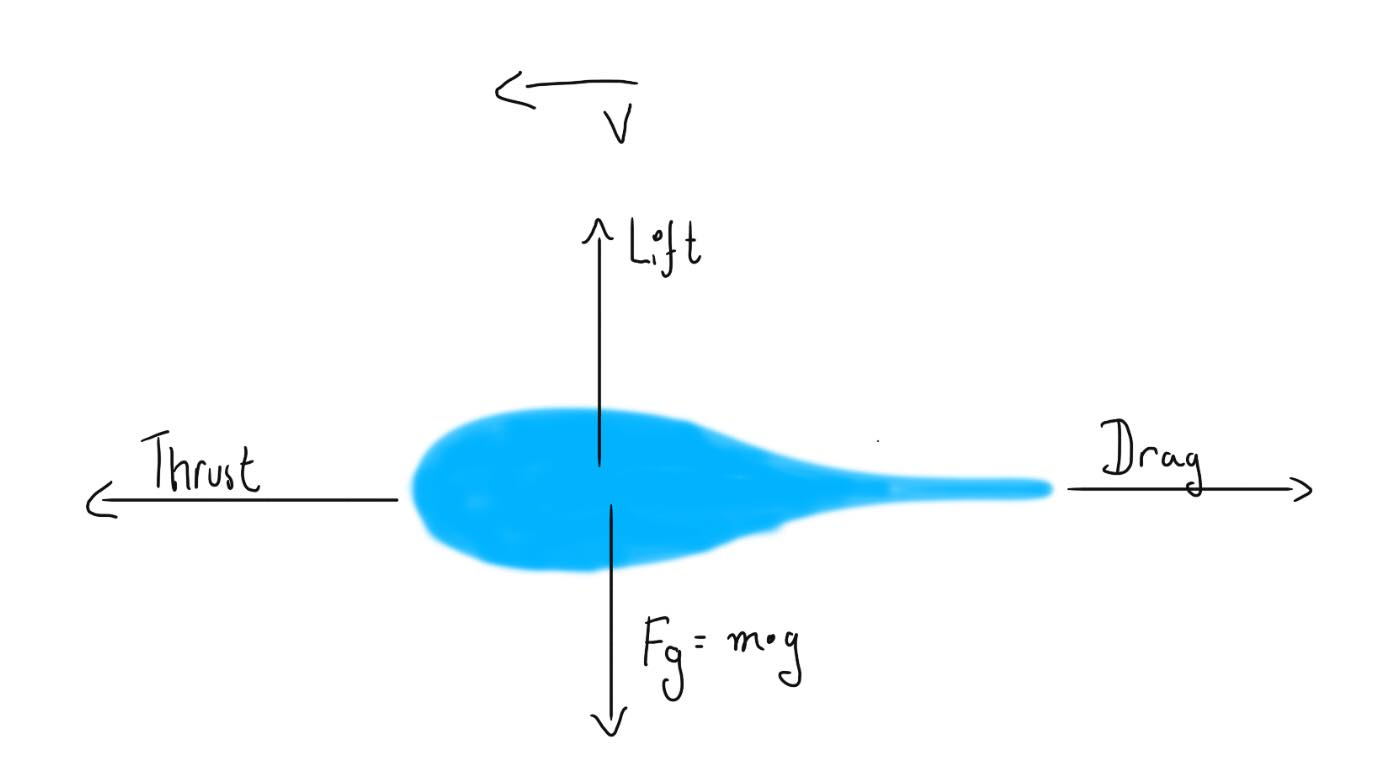
\includegraphics[width=\textwidth]{images/Free_body_teardrop.jpg}
~\label{fig:freeBodyDiagram}
\end{figure}



\subsection{The origin and behaviour of aerodynamic forces}
\textbf{Thrust}: Thrust is the force that pushes a physical object to move in the direction it is applied. It can be from a car's engine or a jet engine.\\
In an airplane, the propeller sucks air from the front of the plane and exerts it behind the propeller, which creates a high pressure area behind the propeller and low pressure in front of the propeller.
This pressure difference pushes the plane ahead.

In cars, the Internal Combustion Engine (I.C.E) applies a torque to the wheels, and due to Newton's III law and traction on the road, the car moves in a specific direction. 
\bigbreak{}

\textbf{Downforce/Lift}: Downforce and Lift are forces of the same origin but acting in different directions.
Lift is actually caused by introducing a shape into a streamlines airflow, which curves the airflow and introduces pressure difference. Low pressure on the upper surface
and high pressure on the lower surface pulls the object upward.~\cite{lift}\\
Just like how wind flows below the object, it also flows above the object but stays attached to the surface due to the coanda effect. The coanda effect is the tendency of a fluid to stay attached to a convex surface can be seen

Downforce is observed due to the pressure below the object is lower than above, which pulls the object downward.
Downforce can simply be achieved by turning the wing upside down. \\


The formula for downforce is
\begin{equation}   
F_{DF}=\frac{1}{2}C_{DF}\rho Av^2 
\end{equation} 
where $F_{DF}$[$N$] stands for the downforce. $\rho$[$\frac{kg}{m^3}$] is the density of the fluid interacting with the object. $C_{DF}$ is the coefficient of downforce,
and $v$[$\frac{m}{s}$] is the relative speed of collision of the object with the medium. $A$[$m^2$] is the cross-sectional area of the object. This formula is derived from the formula for lift since they are the same force in different directions~\cite{5}.
\\\\
\textbf{Drag}: Drag can be thought of as aerodynamic friction. Drag is the force that acts in a direction opposite to the object's motion and is created by the difference in air pressure between the front and the rear of the car.
It slows the car down and makes it difficult to maintain high speed.\\
Streamlined air can be thought of as a medium with multiple layers. When an airfoil is introduced into this streamlined airflow, the air particles in contact with the object will slow down due to frictional forces. 
This causes the second layers which is in contact with the first layer to slow down, but to a lesser extent. Every next layer would follow the same trend.
This effect is illustrated in \textit{figure~\ref{fig:dragIllustration}}, where the more dotted the line is the slower that layer of air is. A CFD simulation (see \textit{section~\ref{sec:CFD}}) of this effect can also be seen in \textit{figure~\ref{fig:teardropV}} where the gradient from red to blue represents the dotted line in \textit{figure~\ref{fig:dragIllustration}}.
This continues until the speed of a layer is the same as before an airfoil was introduced.\\
%The image below shows how streamlines wind flows under the airfoil. The more dotted the line is the slower that layer of air is.

The formula for drag is the similar as the equation for downforce
\begin{equation}   
F_{DR}=\frac{1}{2}C_{DR}\rho Av^2 
\end{equation} 
except the coefficient $C_{DR}$,which stands for the coefficient of drag~\cite{3}.
\begin{figure}[H]
    \caption{Effect on streamlined flow [left to right] upon the introduction of an airfoil, the more dotted the line the lower the velocity of wind} 
    \centering 
    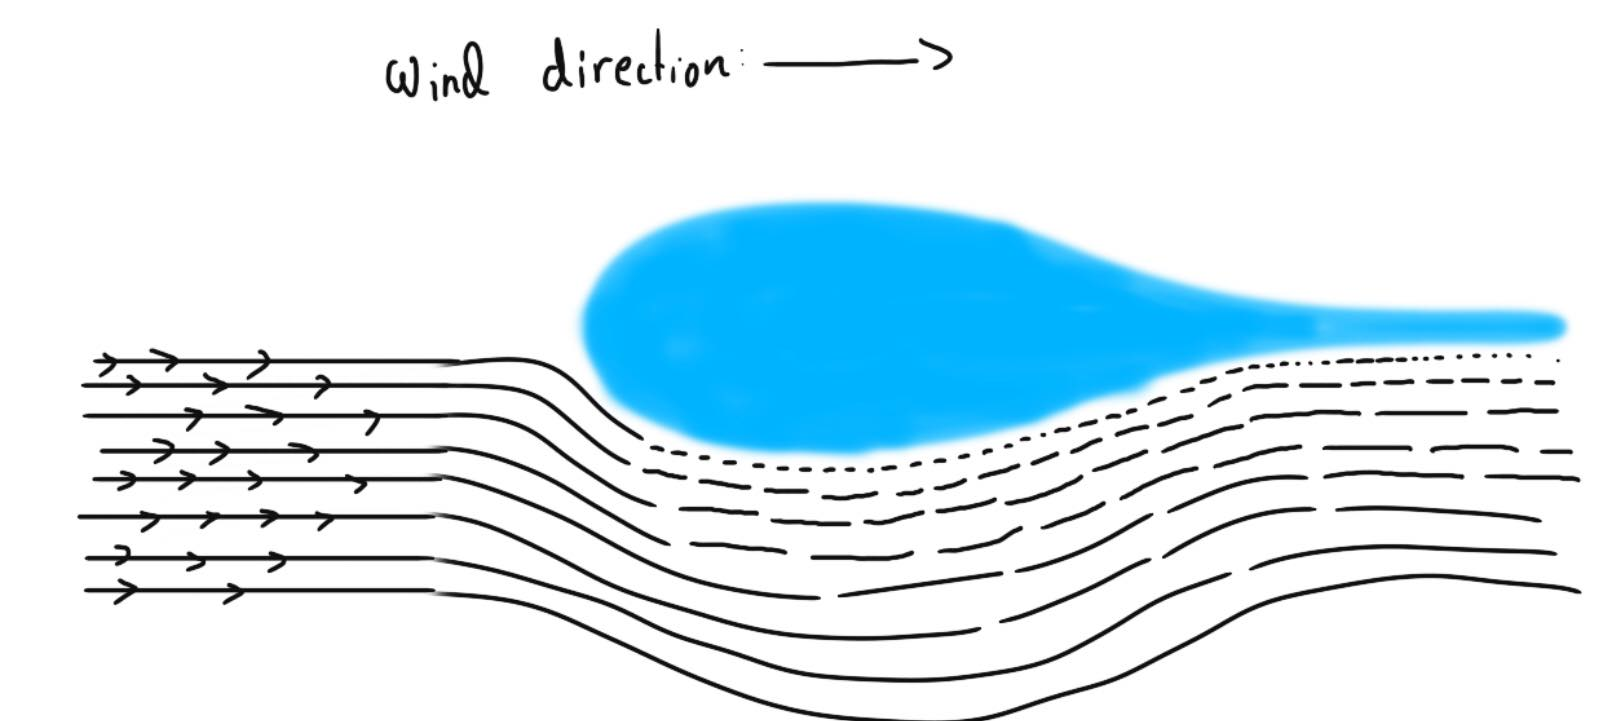
\includegraphics[width=\textwidth]{images/drag_effect_airfoil.jpg}
~\label{fig:dragIllustration}
\end{figure} 

\begin{figure}[H]
    \caption{Simulation of a 2D airfoil in a streamlined airflow. U magnitude is the magnitude of wind velocity} 
    \centering 
    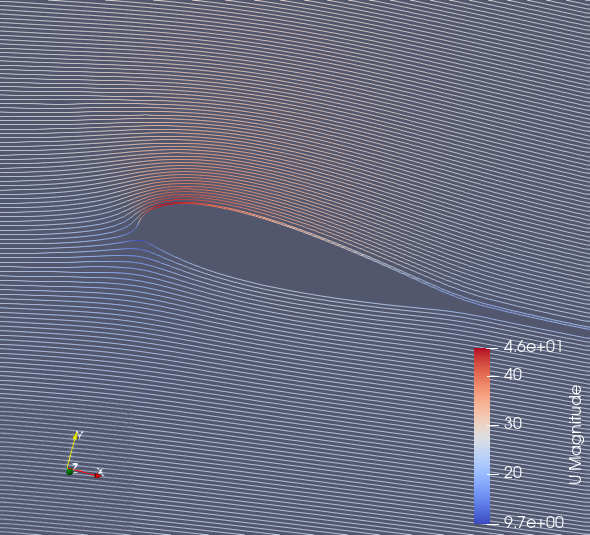
\includegraphics[width=0.7\textwidth]{images/cfd/TearDrop_velocity.png}
~\label{fig:teardropV}
\end{figure}


It should be noted that, this EE uses the aerodynamic interpretation of how forces are generated. Another possible interpretation is using the collision theory, that gas particles will collide with the object more frequently and transfer momentum and thus kinetic energy.
\subsection{Observation of aerodynamic principals in an isolated environment}
For a better visualization of the coanda effect at different AoA, an experimental setup was created. This setup included a water humidifier, a powerful fan and a rear wing from a toy car. The humidifier had an ultrasonic speaker attached to a water reservoir,0 that vibrated to create fine particles of water.
On the other end of the setup, a 12V DC fan was set-up to pull the air with the water particles to create a moderately streamlined flow. A rear wing from a toy car, representing an airfoil, was placed between the fan and humidifier.

\begin{figure}[H]
    \caption{Observation of Bernouli's principle on low (left) and high (right) Angle of Attack} 
    \centering 
~\label{fig:lowHighAoA}
    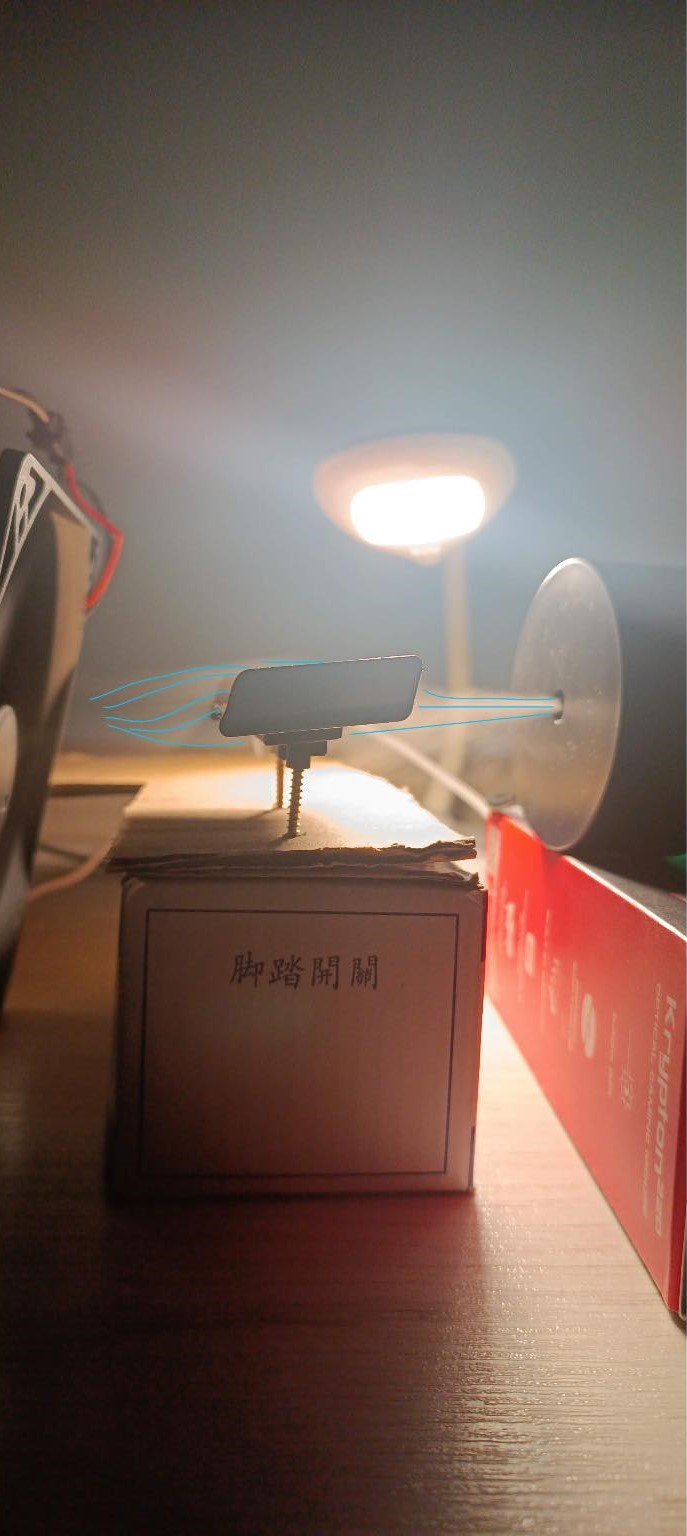
\includegraphics[width=0.4\textwidth]{images/low_downforce_wing.jpg}\hfill
    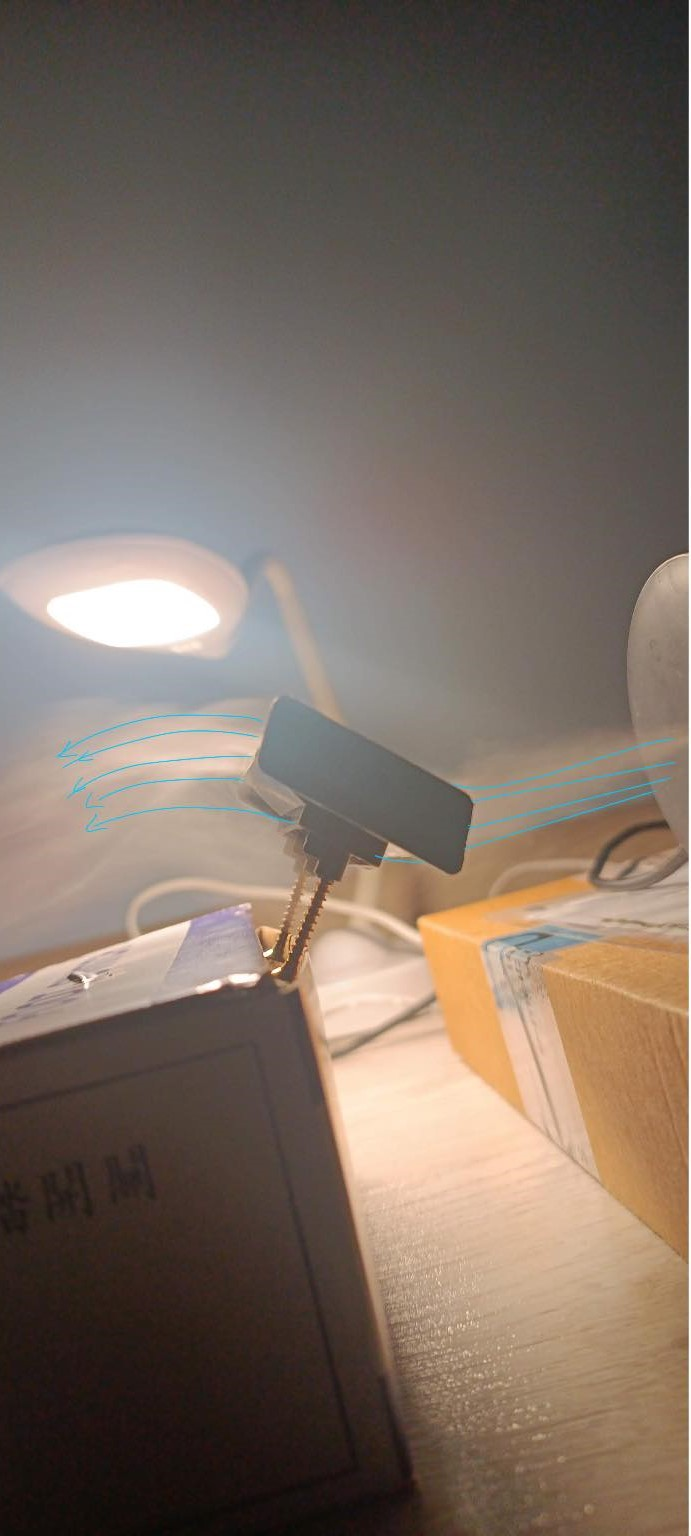
\includegraphics[width=0.4\textwidth]{images/high_downforce_wing.jpg}
\end{figure} 
In the high AoA in \textit{figure~\ref{fig:lowHighAoA}}, the coanda effect. Despite the AoA
the wind follows the curvature of the wind. In \textit{figure~\ref{fig:lowHighAoA}} it is shown that increasing
the AoA creates more disruption in the streamlined flow.

\subsection{Why is angle of attack important?}
The Angle of Attack (AoA) can be increased to create more downforce at the cost of drag, or it could be decreased to create less drag at the cost of downforce. Using high AoA creates a high downforce-drag wing while using a low AoA creates a low downforce-drag wing.
According to a study conducted in 2007\cite{SAE}, there is a significant difference in acceleration and braking between high downforce-drag setups and low downforce-drag setups.
Acceleration was much slower while the braking distance was much shorter~\cite{SAE}~\textit{figure~\ref{fig:SAE}}.
\begin{figure}[H]
    \caption{Difference between No-wing, low-drag-wing and Full-wing, while acceleration and braking~\cite{SAE}[figure 7]} 
    \centering 
    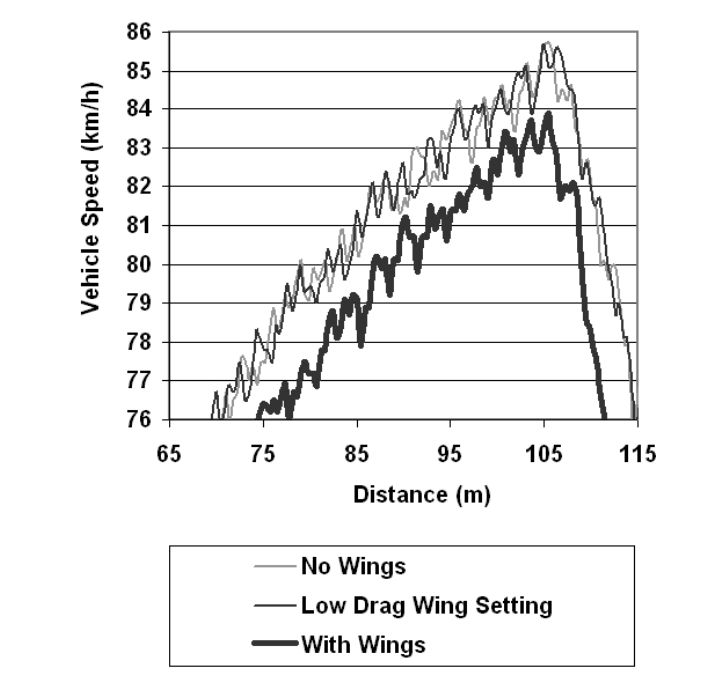
\includegraphics[width=0.7\textwidth]{images/SAE_fig_7.png}
~\label{fig:SAE}
\end{figure} 
Throughout the course of this experiment, the AoA must be a controlled variable as it is heavily influencing the forces acting on the car, which in turn affect the acceleration and velocity.




\newpage{}
\subsection{Computational Fluid Dynamics}~\label{sec:CFD}
Computational Fluid Dynamics or CFD is the process of predicting physical fluid flow by solving the Navier-Stokes equation. The equations are as follow~\cite{9}:
\begin{equation*}   
\nabla \vec{u}=0
\end{equation*}
\begin{equation*}   
\rho \frac{\partial \vec{u}}{\partial t}=-\nabla + \rho \nabla^2\vec{u} + F
\end{equation*}
The first equation just states that the mass should be conserved. The second equation states Newton's $2^{nd}$ law
Using an Open source software called OpenFOAM, these equations can be solved using the help of a computer. These equations have been proven to work with a very high accuracy in many situations as long as the object is a 2D shape.
OpenFOAM runs a program on a 3D object that creates a 2D mesh of the object that wraps around  the 3D object. Using ParaView to visualize the results, the force acting on it at a particular fluid speed can be extracted and compared or in some cases replaced with practical experiments.
\textit{Figure~\ref{fig:turbulence}} shows a CFD simulation demonstration the huge turbulence created by other parts of a car.

\begin{figure}[H]
    \caption{Observation of vortices created by the front wing and the body in CFD simulation} 
    \centering 
    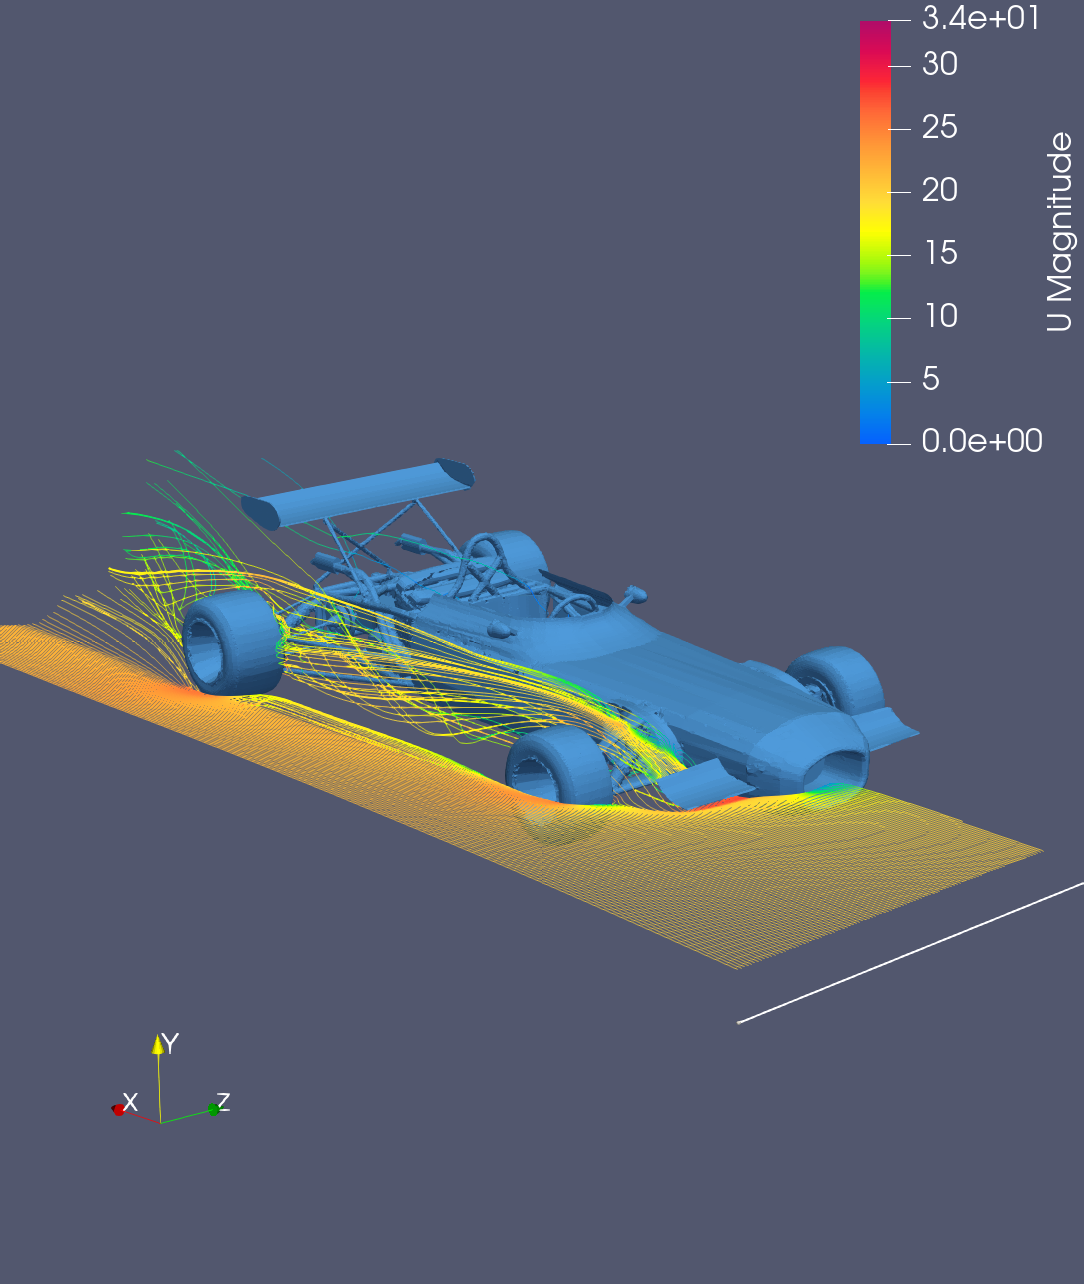
\includegraphics[width=\textwidth]{images/cfd/proofOfWake.png}
~\label{fig:turbulence}
\end{figure} 

For that reason, the rear wing is isolated from other downforce generating structures.

\section{Hypothesis}
According to \textit{Equations (1) and (2)}, the aerodynamic forces increase proportionally to $v^2$ (given $v$ is sufficiently large), of the object at a fixed AoA. As $F_{DF}$ increases the grip levels of the car should also increase which is
reflected by higher acceleration. 
\section{Methodology}
\subsection{Variables}

\textbf{Independent Variable}: Car velocity, Relative wind speed (RWS) \newline
\textbf{Dependent Variable}: Aerodynamic Forces: Drag force: $F_{DR}$ and Downforce: $F_{DF}$ acting on the rear wing  \newline
\textbf{Controlled Variables}: 
%\begin{itemize}
%    \item \gls{AWS}: Variable wind speed induces inconsitent change in aerodynamic forces. A constant wind speed throughout each simulation allow it to be comparable to the car speed.
%    \item Tire temperature and pressure: Tires with higher temperature and/or lower pressure have higher traction on the road, which affects the change in velocity and thus dissalows for an isolated comparison of downforce and velocity. 
%    \item Tire compound: Some compounds are softer than others. The softer compound allows for higher traction which leads to a non-isolated change in velocity.
%    \item Air temperature and humidiy: The temperature and humidity greatly contribute to the density of air. Dense air is generaly harder introduces higher drag than less dense air.
%    \item Elevation: The aerodynamic forces are not isolated as the gravitation force slows down or speeds up the car.
%\end{itemize}
\begin{itemize}
    \item Absolute wind speed (AWS): Variable wind speed induces inconsistent change in aerodynamic forces. A constant wind speed throughout each simulation allow it to be comparable to the car speed.
    \item The grip level of the car that are affected by factors other than downforce can influence the progression of velocity over time. Factors that can affect grip level are \textbf{Tire compound}, \textbf{Tire Temperature} and \textbf{Tire Pressure}.
        These variables were kept constant throughout the experiments. Changes in these variables between trials hampers the comparison of downforce and velocity.
    \item Although evolution of $F_{DR}$ and $F_{DF}$ over time is expected to be similar, the ranges of these variables can be influenced by factors such as air temperature and humidity. 
        Higher car body temperature increases the Drag coefficient of the body which influences the magnitude of the resultant force~\cite{6}. Additionally, higher humidity (density of air) and changing altitude (change in air pressure) results in increased magnitude of the drag force. 
\end{itemize}
\subsection{Simulation Software 1: Assetto Corsa (AC)}
Software:~\cite{7} parameters: \\
\textbf{Car}: Open Wheeler Car, \underline{Mass}: 495kg\newline
\textbf{Aero setup}: Front wing: disabled, rear wing: enabled, $AoA=21.4^{\circ}$\\
\textbf{Driver aids}: Auto clutch\newline
\textbf{Tyres}: Pressure: 12psi, temperature: \(90^{\circ}\)\newline
\textbf{Track Features}: elevation: \(0^{\circ}\), Air temperature: \(26^{\circ}\), Track temperature: \(25^{\circ}\)
\subsection{Simulation Software 2: OpenFOAM}
OpenFOAM~\cite{8} is an open source computational fluid dynamics software. It can simulate, airflow, waterflow, heat flow and electromagnetic fields. This research uses the airflow simulation by simulating a constant wind speed
for 0.3 seconds.

\subsection{Procedure -Data collection from Assetto Corsa}
\begin{enumerate}
    \item A track was chosen which has no turns and no elevation, only a very long straight road. An experiment is done by going from 0km/h to the top speed. A console showing the velocity of the car, the downforce and coefficients ($C_{DF}, C_{DR}$) is displayed.
    \item Set the AWS to \(w_A=0m/s\), every second, the velocity is exported until $t=t_{f}=35s$.  The car reaches the top speed well before $t_f$. Additionally $C_{DF}$ and $C_{DR}$
    \item This simulation is done for \(w_A=4.86m/s\) and \(w_A=7.92m/s\) for which the velocity every second is extracted. The coefficients of Drag and Downforce are also triple checked and confirmed to be constant. 
    \item The car is exported as a 3D object and using OpenFOAM, computational fluid dynamics is performed for a constant wind speed of 20m/s, 30m/s and 40m/s.
\end{enumerate}

\subsection{Procedure -Data collection from OpenFOAM}
\begin{enumerate}
    \item The car from the AC simulation is exported as a Wavefront .obj file.
    \item Using a 3D object editor, only the rear wing of the car is exported.
    \item A new openFOAM project is created where this rear wing .obj file is placed. 
    \item The boundaries of the simulation area are manually defined. And a software is run to create a 2D mesh of the surface of the rear wing.
    \item SimpleFOAM is run to simulate airflow over the rear wing for 0.3s for constant wind speed at 20m/s, 30m/s and 40m/s. This takes about 4 hours to compute.
    \item After computation, the data is opened in paraView to visualize the streamlined airflow. This software also calculates the surface area of the wing, the downforce  and the drag for each wind speed.
\end{enumerate}

\section{Raw Data}
\subsection{Processing of Raw data}
Using equation (1) and (2), knowing the constants and the wind speed, the downforce and drag can be predicted. In this simulation,the fluid is air and the density of air is $\rho=1.293km/m^3$. In the AC simulation when the $w_A=0m/s$, the speed of the fluid is the same as the speed of the car. 
The cross-sectional area would be the same as the surface area of the wing: $A=1.13m^2$. From the AC simulation, it is known that $C_{DR}=0.11$ and $C_{DF}=0.28$. 
Lastly, the acceleration can be calculate using $v(t+1)-v(t)$ for $t$ from 1s-35s. 
\newline \\
The \textit{(Table~\ref{tab:sheet1_excerpt})} shows an excerpt from sheet 1 of the collected data. The rows for Time and Velocity were extracted from the AC simulation, then the Force was calculated using the force coefficients, and acceleration was calculated using $a=v(t+1)-v(t)$.
This table only shows a section of the data collected when AWS=0m/s, but the complete data set contains also the data when AWS=4.86m/s and AWS=9.72m/s. 
\\\\
Note: DF stands for Downforce, DR stands for Drag
\begin{table}[!ht]
    \centering
    \caption{Excerpt from Sheet 1}
    \begin{tabular}{|l|l|l|l|l|}
    \hline
        {Time [$s$]} & {$v [m/s$] ($0 m/s$)} & {$F_{DF}$ [$N$] ($0 m/s$)} & {$F_{DR}$ [N] ($0 m/s$)} & {$a [m/s^2$] ($0 m/s$)} \\ \hline
        0 & 0 & 0 & 0 & \\ \hline
        1 & 0.556 & 0.0630 & 0.0247 & 8.33 \\ \hline
        2 & 8.89 & 16.1 & 6.33 & 6.91 \\ \hline
        3 & 15.8 & 51.2 & 20.1 & 4.50 \\ \hline
        4 & 20.3 & 83.9 & 33.0 & 3.60 \\ \hline
        5 & 23.9 & 116 & 45.8 & 3.90 \\ \hline
        6 & 27.8 & 157 & 61.9 & 2.50 \\ \hline
        7 & 30.3 & 187 & 73.5 & 3.30 \\ \hline
        8 & 33.6 & 231 & 90.6 & 2.50 \\ \hline
    \end{tabular}
~\label{tab:sheet1_excerpt}
\end{table} 
\\
For the seconds sheet: sheet 2, in the first column was velocity from 0-\>225 km/h (Maximum wind speed achieved: top speed of car+ speed of headwind), incrementing every 1km/h. The values were then converted to m/s.
Then using equation (1) and (2), the downforce and drag was calculated. Then using google sheets, an quadratic trendline was computed. And their derivatives were calculated
\begin{equation}
    \begin{split}
        &F_{DF}=0.204v^2-1.05*10^{-3}v+7*10^{-3} \\
        &F_{DR}=0.0802v^2-4.16*10^{-4}v+2.78*10^{-3}
    \end{split}
\end{equation}
\begin{equation}
    \begin{split}
        \frac{d}{dv}F_{DF}=0.408v-1.05*10^{-3}\\
        \frac{d}{dv}F_{DR}=0.1604v-4.16*10^{-4}
    \end{split}
\end{equation}
\begin{equation}
    \Delta \frac{dF}{dv}=\frac{d}{dv}F_{DF} - \frac{d}{dv}F_{DR}
\end{equation}
equations 2, 3 and 4 were also noted into a table.
\begin{table}[!ht]
    \centering
    \caption{Sheet 2: Downforce}
    \begin{tabular}{|l|l|l|}
    \hline
        \textbf{Velocity [m/s]} & \textbf{Downforce [N] t1} & \textbf{Drag [N] t1} \\ \hline
        0 & 0 & 0 \\ \hline
        0.278 & 0.0157 & 0.00619 \\ \hline
        0.556 & 0.0630 & 0.0247 \\ \hline
        0.833 & 0.142 & 0.0557 \\ \hline
        1.11 & 0.252 & 0.0990 \\ \hline
        1.39 & 0.394 & 0.155 \\ \hline
        1.67 & 0.567 & 0.223 \\ \hline
        1.94 & 0.772 & 0.303 \\ \hline
        2.22 & 1.01 & 0.396 \\ \hline
        2.50 & 1.28 & 0.501 \\ \hline
    \end{tabular}
~\label{tab:data2force}
\end{table}
\begin{table}[!ht]
    \centering
    \caption{Sheet 2: Derivatives}
    \begin{tabular}{|l|l|l|}
    \hline
        {$F_{DF}$ Derivative} & {$F_{DR}$ derivative} & {$\Delta$ Derivative($F_{DF}-F_{DR}$)} \\ \hline
        0 & 0 & 0 \\ \hline
        0.112 & 0.0442 & 0.0682 \\ \hline
        0.226 & 0.0888 & 0.137 \\ \hline
        0.339 & 0.133 & 0.206 \\ \hline
        0.452 & 0.178 & 0.274 \\ \hline
        0.566 & 0.223 & 0.343 \\ \hline
        0.680 & 0.267 & 0.413 \\ \hline
        0.790 & 0.311 & 0.480 \\ \hline
        0.905 & 0.356 & 0.549 \\ \hline
        1.02 & 0.401 & 0.618 \\ \hline
    \end{tabular}
~\label{tab:data2_derivatives}
\end{table}

The tables~\textit{~\ref{tab:data2force}} and~\textit{\ref{tab:data2_derivatives}} shows the excerpt from Sheet 2.


\clearpage{}
\section{Data analysis}
From~\textit{table~\ref{tab:data2force}} the graph of forces acting on the wing against the speed of wind was plotted. \\\\
\begin{figure}[H]
    \centering
    \caption{\textbf{Graph of raw values of $F_{DR}$ [$N$] and $F_{DF}$ [$N$] vs car speed [$m/s$] }}
    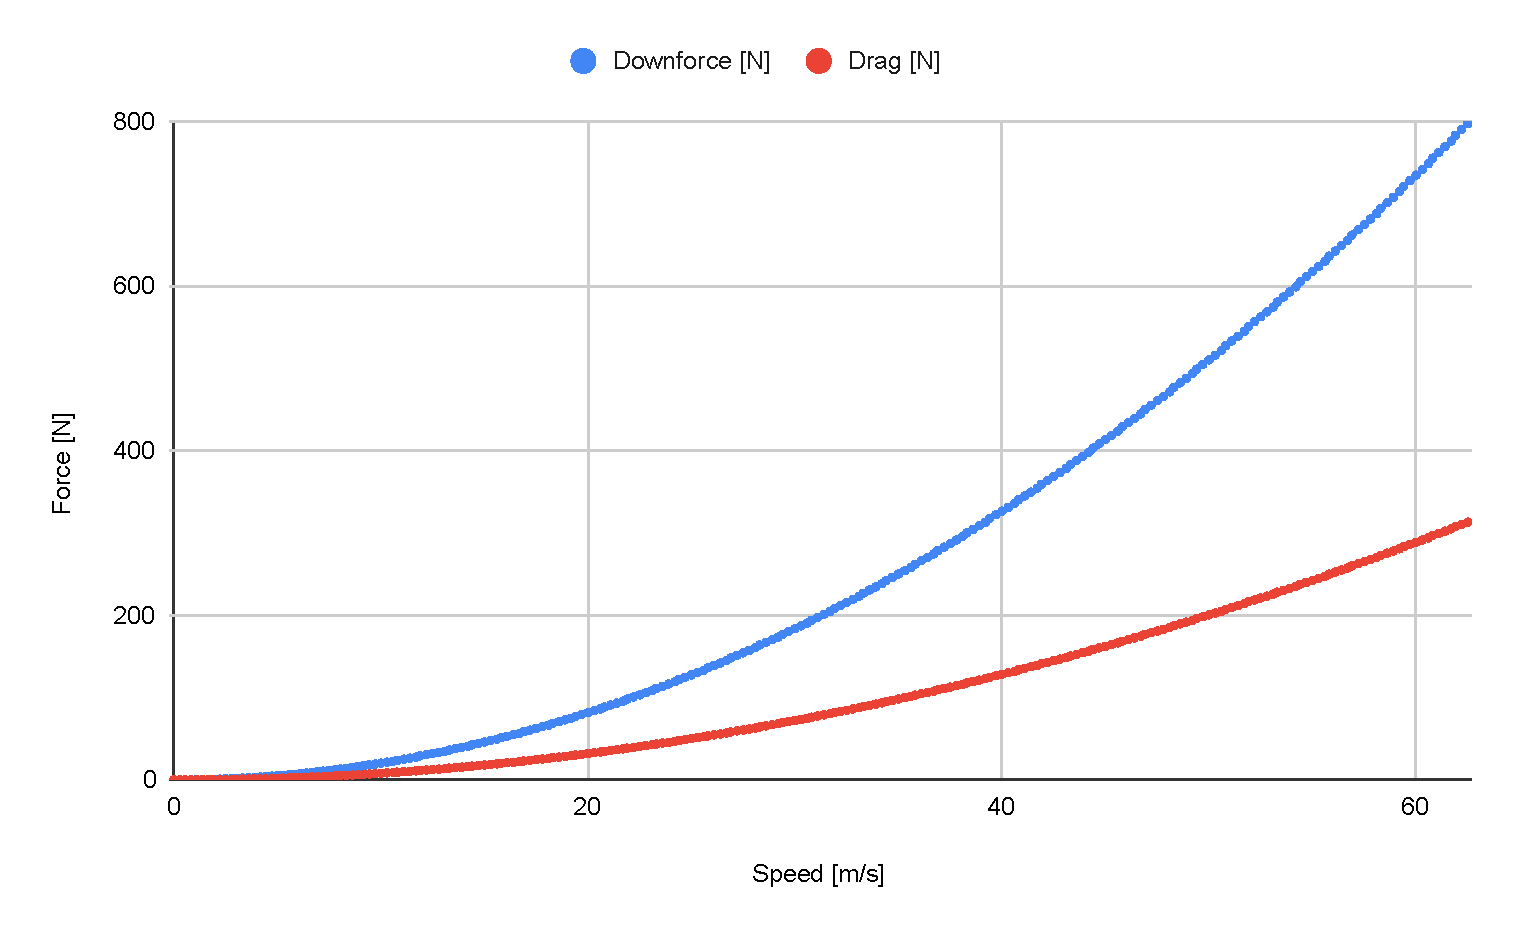
\includegraphics[width=0.82\textwidth]{graphs/DF_DR_VS_VElocity.pdf}
    
~\label{fig:raw_graph1}
\end{figure}
A trendline using Google sheets was plotted with this data. A quadratic trendline was chosen due to equation (1) and (2) of downforce and drag respectively.
\begin{figure}[H]
    \centering
    \caption{\textbf{Graph of trendlines of $F_{DR}$ [$m/s$] and $F_{DF}$ [$m/s$] vs car speed [$m/s$]}}
    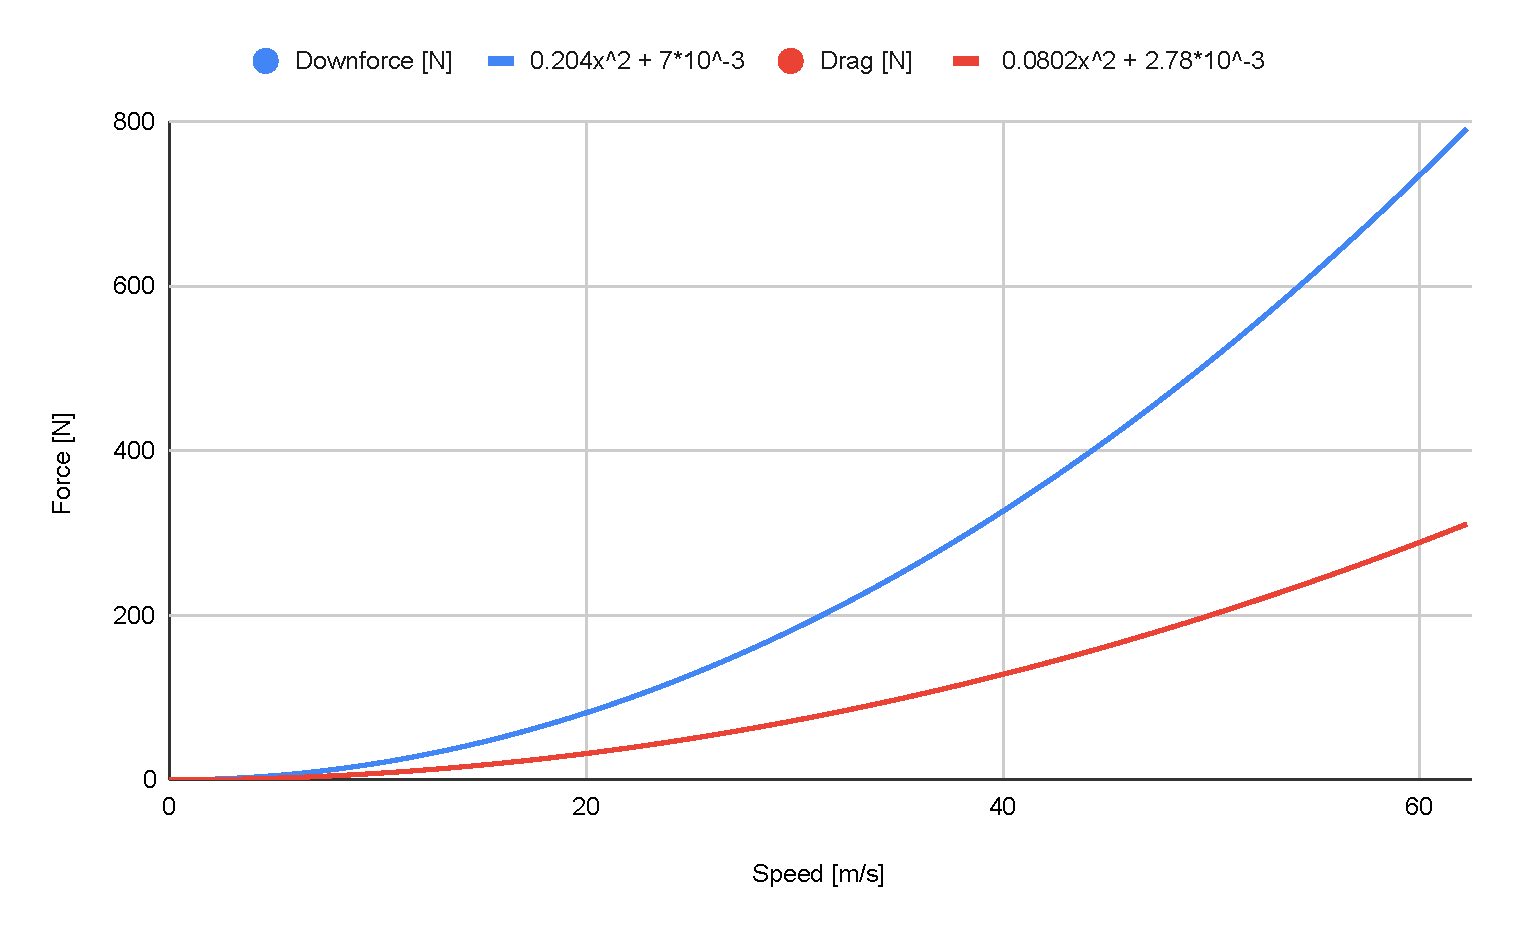
\includegraphics[width=0.82\textwidth]{graphs/DF_DR_VS_VElocity_trend.pdf}
    
~\label{fig:trend_graph1}
\end{figure}
In both graphs~\textit{figures~\ref{fig:raw_graph1} and~\ref{fig:trend_graph1}}, the drag seems to be increasing linearly for small wind speeds. 
This linear velocity dependence happens due to the viscosity of the liquid being the dominant resistive force rather than turbulence. $F_{DF}\propto v$
~\cite{4}
\\
%%But the downforce rises significantly faster than drag. This can be seen by 
Plotting \textit{figure~\ref{fig:der_graph1}} the $\Delta$ Derivatives from~\textit{table~\ref{tab:data2_derivatives}} shows that the rate of change of downforce with respect to velocity, is higher than of drag.
\begin{figure}[H]
    \centering
    \caption{\textbf{Graph of $\Delta$ derivative from }\textit{Sheet~\ref{tab:data2_derivatives}}}
    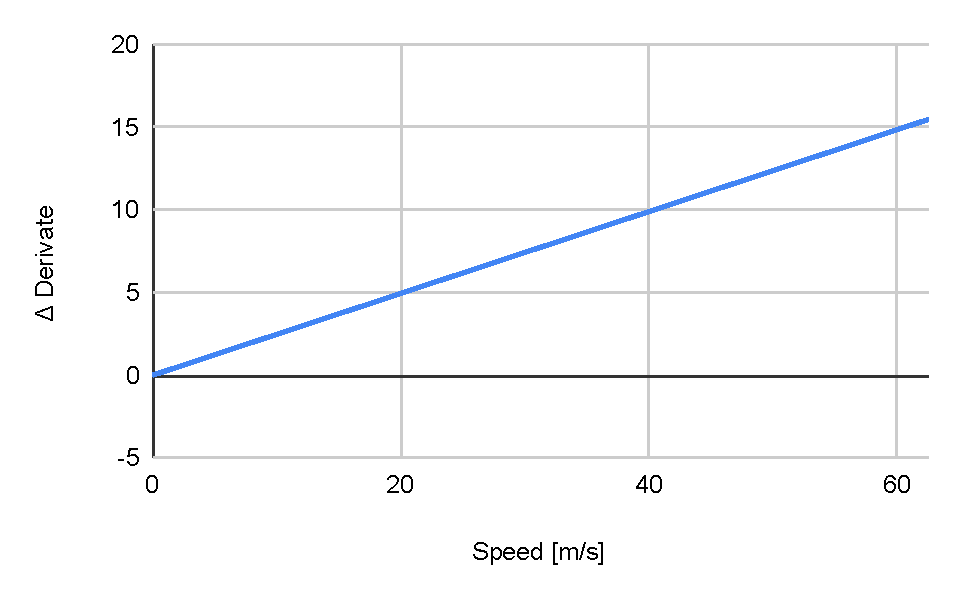
\includegraphics[width=\textwidth]{graphs/D_Der_Speed.pdf}
    
~\label{fig:der_graph1}
\end{figure}

\section{Further analysis}
An increase in $F_{DF}$, results in increased grip, this increased grip results in a higher acceleration. In \textit{(Table~\ref{tab:sheet1_excerpt})},
the last column of acceleration was observed to also be affected by the headwind. The excerpt shows only acceleration for when $AWS=0m/s$, but data for $AWS=4.86m/s$ and $AWS=9.72m/s$ was calculated.
\begin{table}[!ht]
    \centering
    \caption{Excerpt from Sheet 1}
    \begin{tabular}{|l|l|l|l|l|l|l|}
    \hline
        Time [s]  & $a$[$m/s^2$]  ($0m/s$)  & $a$[$m/s^2$] ($4.86m/s$)  & $a$[$m/s^2$] ($9.72m/s$)   \\ \hline
        0  &   &   &    \\ \hline
        1  & 8.33  & 8.06  & 8.03   \\ \hline
        2  & 6.91  & 5.30  & 5.30   \\ \hline
        3  & 4.50  & 3.90  & 4.40  \\ \hline
        4  & 3.60  & 4.10  & 3.70   \\ \hline
        5  & 3.90  & 3.10  & 2.70   \\ \hline
        6  & 2.50  & 3.00  & 3.40   \\ \hline
        7  & 3.30  & 2.80  & 2.20   \\ \hline
        8 & 2.50 & 2.00 & 2.5  \\ \hline
    \end{tabular}
~\label{tab:Accel}
\end{table}

The data from Sheet 1 was plotted and a polynomial trendline was calculated using google sheets.
\begin{figure}[H]
    \centering
    \caption{\textbf{Trendline of Acceleration $a [m/s^2]$ vs. Time $t [s]$ from }\textit{Table~\ref{tab:Accel}}}
    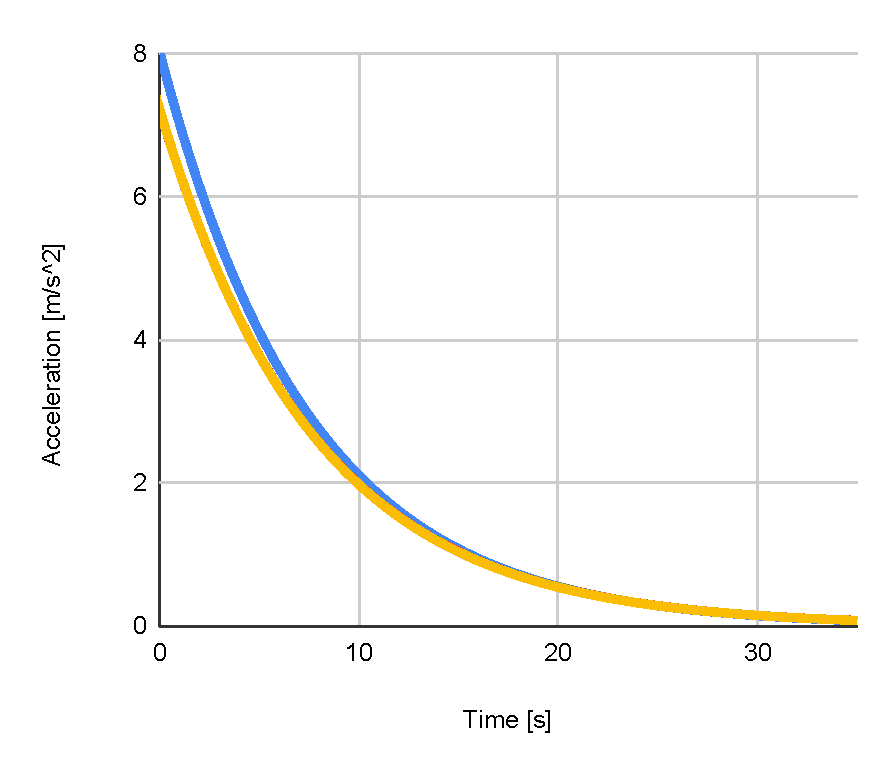
\includegraphics[width=\textwidth]{images/accel.pdf}
    
~\label{fig:accel}
\end{figure}
The graph shows that as the car begins to accelerate, the initial acceleration is higher when the headwind is the lowest ($AWS=0m/s$). As for $AWS=4.86m/s$ and $AWS=9.72m/s$ the progression of acceleration over time is similar.
The reasons for these results are likely due to increased drag. Higher headwind speeds increase the drag component of the force. Although I was expecting this effect to be counterbalanced by the increased grip, it seems that the drag component was dominant.
\\\\
The drag and downforce component of the force acting on the car were also analysed against time to identify the rate of change of each. 
\begin{figure}[H]
    \centering\caption{\textbf{Evolution of $F_{DR}$ for different $AWS$ (value in round brackets)}}
    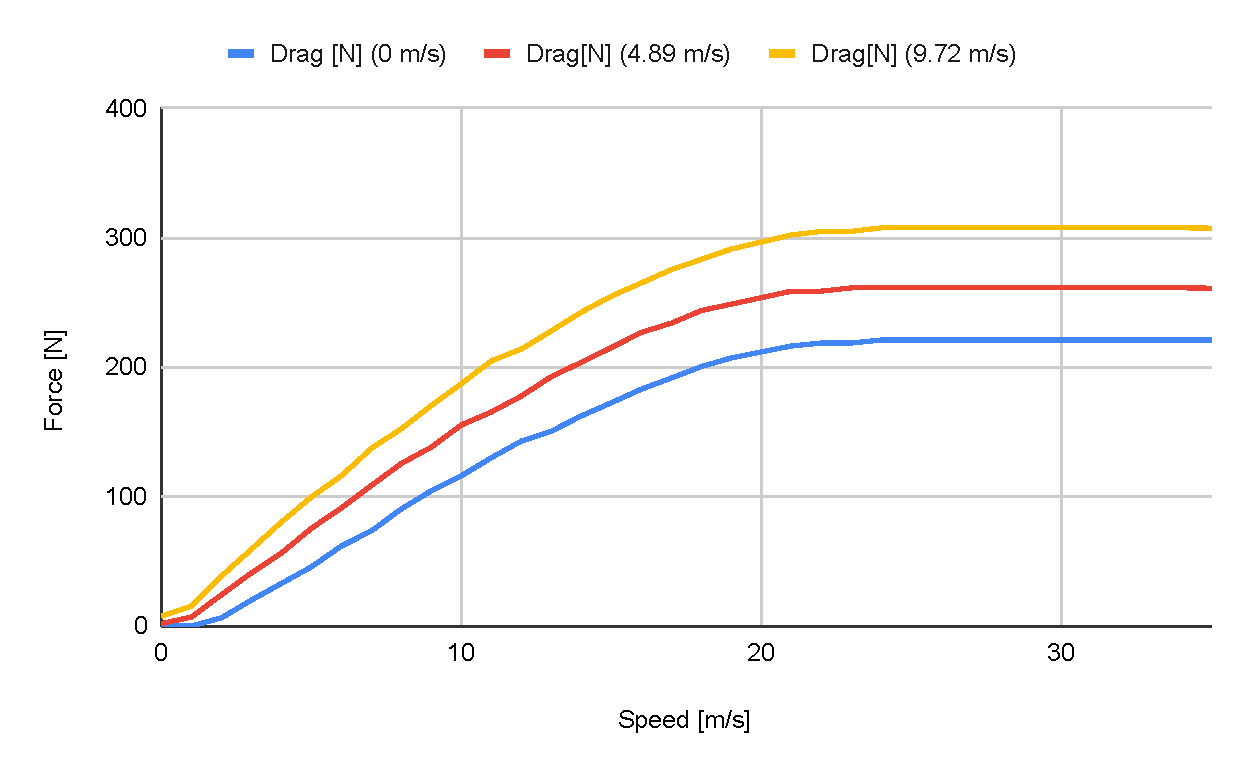
\includegraphics[width=\textwidth]{images/drag_time.pdf}
    
~\label{fig:dr_time}
\end{figure}
\begin{figure}[H]
    \centering
    \caption{\textbf{Evolution of $F_{DF}$ for different $AWS$ (value in round brackets)}}
    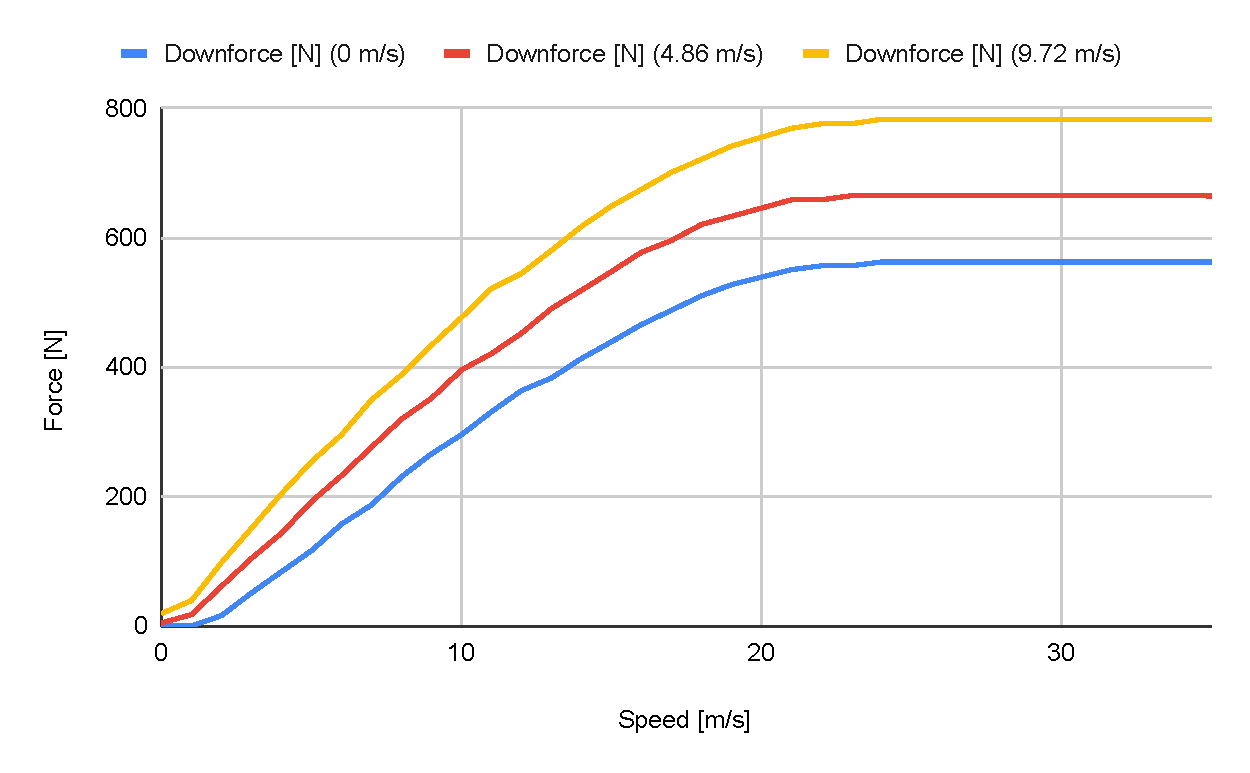
\includegraphics[width=\textwidth]{images/df_time.pdf}
    
~\label{fig:df_time}
\end{figure}
The graphs \textit{{graph~\ref{fig:dr_time} and~\ref{fig:df_time}}}, show how at different headwinds the downforce changes over time. For $AWS=0m/s$ the drag is the lowest, while for $AWS=9.72m/s$ the drag is the highest.
A similar trend is observed for downforce where the speed of the headwind seems proportional to the rate of change of downforce and maximum downforce.
This explain the findings for why acceleration was similar for $AWS=4.86m/s$ and $AWS=9.72m/s$. The is likely due to the grip starting to play a more dominant role. 
\section{Conclusion}
The analysis of the data above show that both drag and downforce, increase linearly for very slow speed but for higher speeds the force increases quadratically. This shows that if a driver wants
to utilize the full aerodynamic capabilities of their car then they must go fast. This suggest that if a drivers were to drive at 10m/s and brake down to 1m/s for a turn, they would be slower than if they drove at 20m/s and would brake down to 2m/s. Since the downforce would 
provide a significant amount of downforce the cars have more grip as they go faster, and are able to take the turn at higher speeds.
\\\\
Another conclusion is that since the rate of change of downforce is higher than the rate of change of drag, the manufacturers should set up the wing with a higher~\gls{AoA}, as that would increase downforce.
This strategy can only be applied to racing circuits such as Monaco and Zandvoort. This is because, in such circuits with lots of turns and small straights having higher downforce can lead to taking turns faster and hence overall lap times. 
The drag is less prioritized since taking the corners faster is more beneficial than going faster on the straights.
\\\\
Conclusions devised from the further analysis section, are based on speculations. These findings lead to the hypothesis that after a certain threshold of headwind speed, the higher $AWS$ is, the faster the car accelerated initially.
To confirm these findings, experiments with higher headwinds must be performed. This is out of the capabilities of Assetto Corsa as the simulation allow up to $AWS=9.72m/s\approx35km/h$. Although, racecars are likely to not race in such extreme speeds
due to safety reasons, headwind higher than these are achieved when as the car gains velocity. As then the headwind would be equal to the $AWS$ + the car's velocity.

\section{Evaluation}
This experiment was performed under idealistic conditions, such as non-turbulent air, which resulted in certain strengths and limitations.
\\\\
One strength of this research was the use of researcher triangulation. 
To show the Bernoulli's effect on a wing, an experimental wind test was performed to show the theory working in practice, 
and a CFD 2D airfoil experiment was performed to numerically show the Bernoulli's principal.
\\\\
Another strength was the use simulations. 
As calculations are done by the computer, multiple times per second, the accuracy of data is high enough for the propagation of uncertainty withing a particular simulation is low enough to be disregarded.
Additionally, due to the theoretical nature of the experiment the experimental conditions were controlled to a high degree. This allowed for a clear cause and effect to be observed.
\\\\
%Thirdly, the methodology of this experiment has high replicability due to the easy of access to simulation softwares.
%The conclusion of this experiment are consistent with what motorsports have been doing in practice. The racers have been observed to drive at a certain minimum speed to utilize the aerodynamic capabilities of the car.
%Certain formula 1 teams have opted for a car that generates high downforce at the cost of drag. 
There are also several limitations to this experiment.
\\
Firstly, there is a small risk of circular reasoning. The formulas deduced from the AC simulations might have been the formulas used to make this simulation. Due to AC being a closed source simulation, this cannot be verified.
This is likely to not be the case in OpenFOAM, as it utilizes the Navier-Stokes equations, which is quite unlikely for Assetto Corsa to be able to calculate in real time.
\\\\
Secondly, the assessment of uncertainties is difficult to make without comparison to real life values through performing experiments or evaluating other research. Performing an on track experiment requires a lot of finance and time.
The experiments done by other motorsports teams aren't published due to their proprietary nature. This creates a lack of literature values to compare to.
\\
Albeit the lack of literature values to compare to, it can be assumed that CFD experiments are comparable to real life experiments to a certain degree. In~\textit{(section~\ref{sec:uncertainties})}, these uncertainties are calculated and compared



\subsection{Quantitative Uncertainties} \label{sec:uncertainties}
Performing a streamlined flow of air experiment using CFD on the rear wing of the car chosen, the downforce $F_{DF}$ and drag $F_{DR}$ on the wing were calculated. The 3 different wind speeds were 20m/s, 30m/s and 40 m/s. 
The uncertainties were calculated using the following formula:
\\
\begin{math}
    err\%=\big|\frac{theo-exp}{theo}\big| * 100\%
\end{math}
\\
The theoretical values $theo$ are from the Assetto Corsa simulation from~\textit{sheet~\ref{tab:data2force}} and the experimental values $exp$ are from CFD.
Then the average of 3 uncertainties $err\%$ was taken:
\begin{table}[!ht]
    \centering
    \begin{tabular}{|l|l|l|}
    \hline
        \textbf{} & \textbf{Downforce} & \textbf{Drag} \\ \hline
        \textbf{Average Uncertainty \%} & 9.46\% & 2.65\% \\ \hline
    \end{tabular}
\end{table}
\\\\
This error data can be plugged into the graph~\textit{figure~\ref{fig:trend_graph1}} to get the error zone of the forces acting on the wing.
\begin{figure}[H]
    \centering
    \caption{\textbf{$F_{DF} [N]$ and $F_{DF} [N]$ vs Speed [$m/s$] with a zone of error}}
    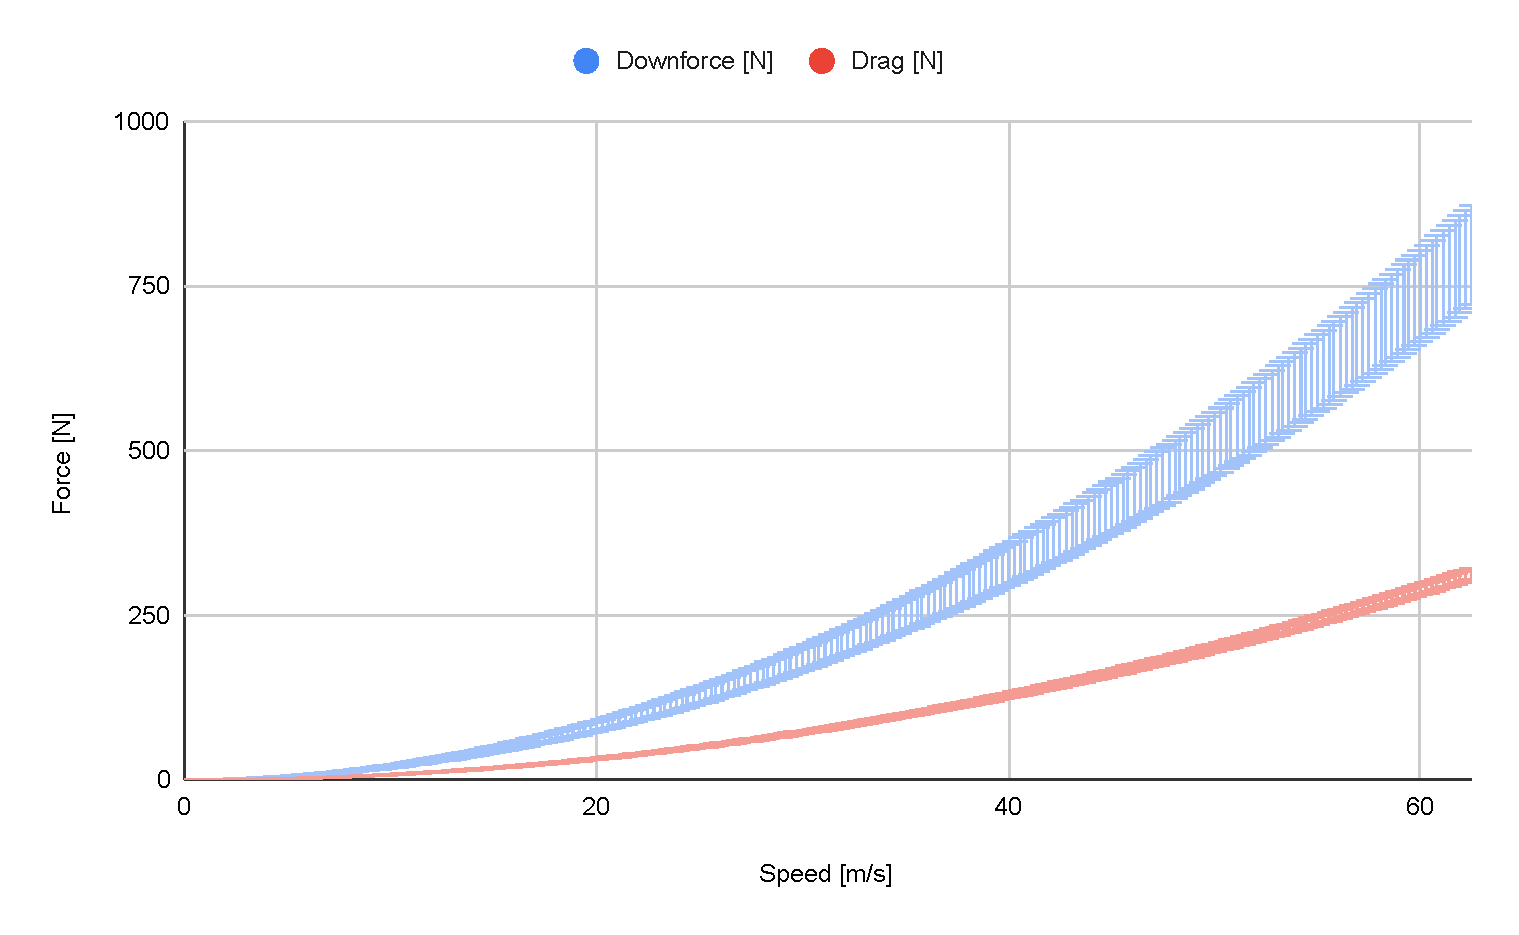
\includegraphics[width=0.9\textwidth]{graphs/DF_DR_VS_VElocity_error.pdf}
    
~\label{fig:err_graph1}
The c
\end{figure}
The blue and red areas show the error region of the downforce and drag at a particular velocity. 
This accuracy difference could be due to a number of reasons. One reason is the optimization of Assetto Corsa. The 3 CFD simulations took up 
ito 12 hours, while Assetto Corsa does the calculations in real time.
%It is very unlikely, that Assetto solves the Navier Stokes equations in real time, but instead has pre-trained models that are optimized to run in real time. This optimization might be at the cost of accuracy.
%Kunos Simulazioni, the creators of Assetto Corsa, also create a version of the game for racing teams that is not optimized to run on lower end PCs but run only on clusters of PCs. 
The increased speed of calculations could be at a cost of accuracy. Since, Assetto Corsa is a closed source software, only assumptions of its mechanisms can be made. One such assumption is that AC uses pre-trained models
that are optimized to run in real time. 

Another reason for the uncertainties could be attributed to human error. When the researcher was driving the car, they tried to keep the car in a straight line, but minor hand movements might have cause the car to go slightly diagonally.
In this situation the headwind turns to a crosswind. This could explain the relatively small uncertainty observed, as the car moved diagonally for very little time and distance.

\subsection{Qualitative Uncertainties}
Apart from Quantitative Uncertainties, there are many other factors than can introduce an uncertainty in the handling and performance of the car. In a real life race scenarios, the race track goes through multiple 
altitude changes which results in difference in air density and gravitation play a more important role in grip level at certain parts of the track. Additionally, the track and air temperature are likely to change throughout the course of
the race. Since air temperature is a direct measure of the Kinetic energy of air particles, variations in magnitude of forces can be observed. 

This EE assumes ideal conditions where variables like humidity and elevation are kept constant. In practice, the controlled variables in this EE are not constant

Experiments such as one performed in this research, allow the teams to understand the potential of their car. This experiment only measures airflow with headwind, whereas professional teams that have the resources and time, perform experiments multiple directions of wind, with different air densities
and different temperature conditions. This narrows down the uncertainty window and allows for a more predictable behaviour from the car. 

%\subsection{Benefits to Real life:}
\subsection{Possible Improvements}
%One possible reason \textbf{Quantitative Uncertainties} is the optimization of the simulation software AC. The CFD simulations that took upto 12 hours  of computational time, are performed in real time in Assetto Corsa. Due to such efficiency, it is quite unlikely that AC solves the Navier-Stokes equations
%in real time. Most likely, AC has pre-trained models that are optimized, which would come at a cost of accuracy. 
%One possible solution is to use the enterprise version of Assetto Corsa. This version is very demanding on the hardware it runs on, and requires the user to optimize the simulation for their particular car. This version calculates graphics
%at a higher rate than the base version. Although this wouldn't completely replace CFD, it can provide a much more accurate result.

One improvement that can be made, is performing the experiment for different headwinds with a shorter interval. The \textit{figures~\ref{fig:df_time}} and \textit{~\ref{fig:dr_time}}
are performed only for 3 different $AWS$, whereas performing for more would have allowed for a more accurate trend between the headwind and the rate of change of aerodynamic forces to be observed.

Another improvement can be made to reduce \textbf{Qualitative Uncertainties} by performing the experiment on a real life track with a real vehicle. This can be rather financially and time demanding. Simulating the car in conditions that accurately
reflect real life, comes with a lot of complications. Apart from the huge number of variables and their combinations, the simulation software may not model certain factors like humidity and temperature accurately.

\section{Further research}
The use of simulations and a theoretical approach of this experiment shows that, racing teams can slowly shift towards completely simulating their race cars by creating simulation models that reflect real life conditions.
Although creating such models is very time consuming, once its results are assessed and are fine-tuned to reflect real life, manufacturers can save resources by eliminating the need
to test in wind tunnels. This could greatly benefit the environment and also promote technical advancements.


\clearpage
%\printnoidxglossaries{}
\printbibliography{}
\end{document}
